% !TEX root = ../example_paper.tex

\section{Contexto}

Nesta seção, discutimos inicialmente conceitos relacionados a BI, com destaque para modelagem dimensional e ETL. Em seguinda, detalhamos como o TRE-RN faz uso de técnicas de BI no seu cotidiano, abrangendo tanto o contexto eleitoral como sua gestão interna. Por último, aprofundamos a discussão sobre o processo de ETL no contexto do tribunal, foco de nossa investigação.

\subsection{Business intelligence (BI)}

\textit{Business intelligence}~\cite{BI} é a agregação de valor de negócio a uma empresa ou organização a partir de seus dados. Técnicas de BI permitem, por exemplo, a exibição de informações de forma mais interpretável para gestores, auxiliando na tomada de decisões e no monitoramento de resultados. 

Uma das abordagens de BI mais usadas em bancos de dados é a modelagem dimensional~\cite{artmodelagem}. A modelagem dimensional tem como objetivo a transformação dos dados do modelo entidade-relacionamento, tradicional em bancos de dados relacionais, para um modelo usando fatos e dimensões, visando uma melhor performance de leitura. O fato representa a unidade mais granular de um indicador que se deseja medir. As dimensões se referem às informações que se deseja analisar a respeito do fato.

A modelagem dimensional costuma ser operacionalizada por um processo de ETL, onde os dados são coletados, integrados e tratados para que possam ser persistidos no formato desejado~\cite{etl}. A extração é a primeira parte do ETL e tem como objetivo a coleta de informações oriunda de (potencialmente) diversos tipos de bases de dados. A transformação tem como objetivo integrar os dados e tratá-los, corrigindo erros e mudando sua organização, por exemplo. Por último, os dados tratados são injetados em um novo repositório para que possam ser analisados posteriormente.

\subsection{BI no contexto do TRE-RN}

O TRE-RN é um órgão do Poder Judicário responsável pelo processo  eleitoral de todas as 60 zonas eleitorais do estado do Rio Grande do Norte~\cite{zonas}. Em 2018, por exemplo, o RN totalizava 2.373.619 eleitores em seus 167 municípios~\cite{eleitorado}, cujo registro e acompanhamento é feito pelo TRE-RN. Para lidar com esta demanda, o TRE-RN apresenta uma equipe de cerca de 600 servidores, distribuídos pelas zonas eleitorais do estado~\cite{servidores}. Assim, apesar de dispor de uma grande quantidade de informações, esses dados encontram-se dispersos nos mais de 50 sistemas implantados no TRE-RN, segundo a Coordenadoria de Sistemas Corporativos da Secretaria de Tecnologia da Informação e Comunicação do TRE-RN.
% , por esse motivo o processo de BI é necessário.
% No TRE-RN, essas informações se referem a informações de eleições, cadastro eleitoral e gestão do Tribunal.

Os sistemas existentes no tribunal perpassam propósitos variados, como gestão de pessoas, orçamento e cadastro eleitoral. Com isso, existe uma grande variedade de bases e tipos de dados no tribunal. Os principais bancos de dados utilizam o sistema de gerenciamento de bancos de dados (SGBD) \textit{Oracle}~\cite{}. Adicionalmente, informações estruturadas podem estar armazenadas em planilhas \textit{Excel}, arquivos CSV (\textit{comma-separated values}), ou em bancos de dados que usam o SGBD \textit{PostgreSQL}. Por fim, há também informaçãos não- ou semi-estruturadas, como arquivos PDF ~(\textit{printed document file}). 

O processo de BI no TRE-RN utiliza uma estrutura comumente adotada na literatura e no mercado, mostrada na Figura~\ref{fig:galaxy}. Especificamente, o processo de ETL processa as informações espalhadas nas diferentes fontes de dados e as persiste em um \textit{data warehouse}~(DW). \textit{Dashboards} que se alimentam deste DW permitem o monitoramento de processos por parte de servidores e auxiliam na tomada de decisão por parte de gestores. As ferramentas utilizadas no TRE-RN em cada uma destas etapas são descritas a seguir:

\begin{figure}[htp]
    \centering
    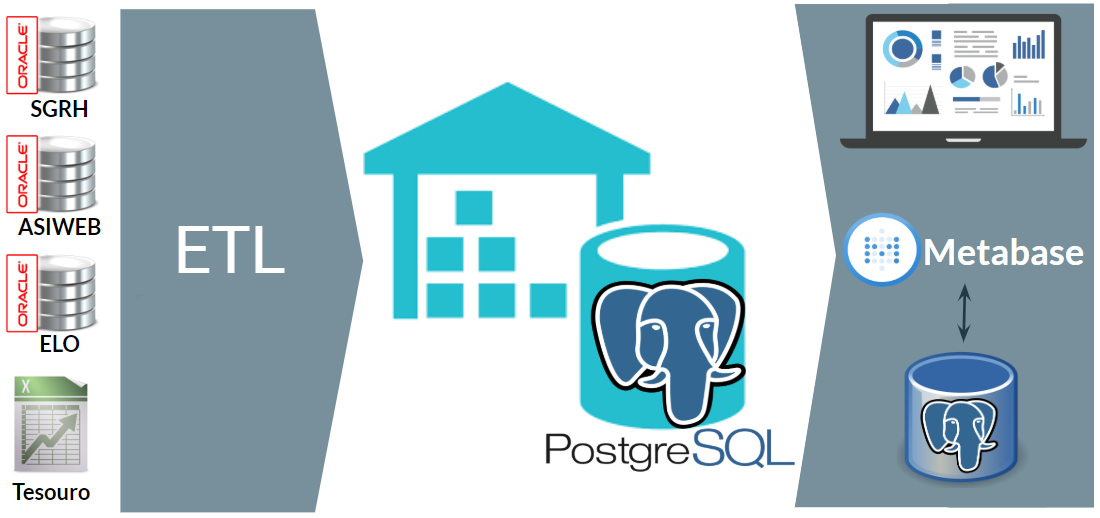
\includegraphics[width=8cm]{Imagens/Arq_TRE}
    \caption{Arquitetura de BI no TRE-RN.}
    \label{fig:galaxy}
\end{figure}

\textbf{Pentaho Data Integration}~(PDI) é uma ferramenta de código aberto da \textit{suite} Pentaho~\cite{pentaho}, responsável pela extração e tratamento dos dados disponíveis em fontes de dados estruturados, como bancos de dados relacionais e planilhas. O PDI modela processos de ETL como transformações e \textit{jobs}~(\textit{workflows}). Uma transformação é um conjuntos de operações de coleta e tratamento de dados. Um \textit{workflow} reúne uma ou mais transformações, definindo a ordem em que elas acontecem e eventuais dependências entre transformaçòes.

\textbf{Apache Tika} é uma ferramenta de código aberto da Apache Software Foundation (ASF, \citet{apache}) que extrai metadados de diversos tipos de arquivos de texto, como arquivos PDF. No contexto do TRE-RN, o Apache Tika é usado para a extração de informações de arquivos PDF de faturas de água e energia.%, usadas para comprovação de residência no cadastro eleitoral.

\textbf{CRON} é uma aplicação UNIX usada para agendamento de tarefas~\cite{cron}. Apesar de ser bastante utilizada em servidores Linux, é uma ferramenta bastante simples por seguir a filosofia UNIX ``\textit{do one thing well}"~\cite{unix}. O TRE-RN utiliza o CRON para agendar a execução de \textit{workflows}, como será detalhado adiante.

\textbf{PostgreSQL} é um sistema gerenciador de banco de dados (SGBD) relacionais de código aberto~\cite{postgres}. Compatível com o paradigma ACID~(atomicidade, consistência, isolamento e durabilidade), o PostgreSQL é conhecido dentre outras coisas por seu suporte nativo a dados georeferenciados. No TRE-RN, o PostgreSQL é o SGBD usado para gerenciar o DW produzido como resultado do processo de ETL. 
% é o repositório que foi decidido para ser usado como DW. Neste banco de dados as grande áreas são divididas por esquemas e os nomes das tabelas definem a subárea e o tipo da tabela.

\textbf{Metabase} é uma ferramenta de código aberto de visualização de dados~\cite{metabase}. Além de permitir a construção de \textit{dashboards} baseados em consultas a bancos relacionais, o Metabase permite a disponibilização de \textit{dashboards} em formato Web para consulta em \textit{desktops} e dispositivos móveis.

\subsection{ETL no contexto do TRE-RN}

No TRE-RN, as informações utilizadas no BI devem ser atualizadas diariamente, permitindo que os servidores do tribunal possam extrair relatórios ou visualizar a situação atual ou pretérita dos processos do tribunal. O ciclo de vida dos \emph{workflows} de ETL usados para manter essas informações atualizadas consiste de quatro etapas, detalhadas a seguir:
%No TRE-RN, as informações visualizadas devem estar sempre atualizadas com o dia anterior, permitindo que os servidores do tribunal possam extrair relatórios ou visualizar a situação atual ou pretérita dos processos do tribunal. A partir disso, para que possamos realizar o processo de ETL de forma completa, precisamos realizar três etapas: estudo das bases de dados, criação dos \textit{jobs}, injestão dos dados no DW, agendamento dos \textit{jobs]} no CRON e visualização no Metabase.

\begin{enumerate}
\item \textbf{Delimitação das fontes de dados}: o TRE-RN reúne sistemas desenvolvidos localmente no RN e sistemas desenvolvidos a nível nacional pelo Tribunal Superior Eleitoral (TSE). Para definir as consultas necessárias para uma modelagem dimensional, é necessário identificar quais tabelas e bancos de dados armazenam as informações desejadas. Este processo é operacionalmente custoso, uma vez que um único banco chega a apresentar mais de 200 tabelas. Além disso, parte da informação pode ser oriunda de fontes não- ou semi-estruturadas, como discutido anteriormente.
%Nessa etapa fazemos o estudo das tabelas existente na base de dados selecionada. Devido a robustez dos sistemas existentes do TRE-RN, esse processo se tornar demorado pela grande quantidade de tabelas existentes, com esse número podendo chegar a mais de trezentas tabelas.

\item \textbf{Criação}: o PDI e/ou o Apache Tika realizam a extração das informações necessárias a partir das fontes de informação identificadas na etapa anterior. Especificamente, o Apache Tika é encapsulado por \emph{scripts} Python, uma linguagem com a qual os servidores do TRE-RN já têm familiaridade. Um \emph{workflow} PDI ou Python reúne (potencialmente) múltiplas transformações, realizando (i)~a~extração das informações das tabelas selecionadas; (ii)~o~tratamento e a adequação dos dados para o formato desejado, e; (iii)~a~criação de tabelas e a ingestão dos dados transformados no DW. 
%Nesse processo de transformação sempre usamos a modelagem dimensional para a organização das informações. 
%Após a criação de todas as transformações necessárias, criamos o \textit{job} que executará as transformações na ordem desejada.
%\textbf{Ingestão dos dados no DW}: Com a modelagem deifnida e os dados prontos, realizamos a injestão dos dados no DW. Dentro do DW definimos uma organização de modo que as tabelas sejam dividas em esquemas que representem as grandes áreas do TRE-RN, como cadastro eleitoral, gestão de pessoas, entre outros exemplos.

\item \textbf{Agendamento no CRON}: uma vez validado, a execução do \emph{workflow} é adicionada ao agendamento do CRON 
 %o processo completo através de forma manual, realizamos o agendamento no Cron 
para que possa ser executada de forma automática. No TRE-RN, o agendamento requer um nível restrito de permissão, podendo ser realizado apenas por uma seção responsável. Este é um segundo gargalo operacional no processo, uma vez que o tempo de resposta para este tipo de solicitação varia em função da demanda existente. Em períodos eleitorais, isto pode chegar a inviabilizar a solicitação.
%O agendamento é feito através da adição do comando utilizado para a execução de um job via terminal em um arquivo. Após essa adição, realizamos um pedido a seção do TRE-RN responsável pelo CRON para que o arquivo possa ser agendado.

\item \textbf{Manutenção}: apesar de automatizado,  o \textit{workflow} deve ser monitorado para assegurar que sua execução esteja acontecendo corretamente. Eventualmente, a execução de um \emph{workflow} pode apresentar erros que precisam ser depurados. Isto é feito através da análise do seu \emph{log} de execução. \emph{Logs} de execução de \emph{workflows} PDI são excessivamente verbosos, enquanto \textit{logs} de execução de \textit{workflows} Python podem ser customizados. A correção do erro pode exigir que um \emph{workflow} seja remodelado em relação a uma ou mais das etapas anteriores. 
%\textbf{Visualização no Metabase}: Com o DW contendo todas as informações de forma atualizada, utlizamos o Metabase para a criação de \textit{dashboards} que possam aprensentar as informações de uma forma mais intuitiva. Como forma de organização, utilizamos uma estrutura do Metabase chamada coleções, que tem como objetivo realizar uma divisão através de pastas, para que possamos organizar os dashboards e perguntas em grandes áreas e subáeas, deixando  a utlização da ferramenta mais fácil.

\end{enumerate}

Na seção seguinte, discutiremos as principais ferramentas utilizadas para gerenciamento de \emph{workflows} relacionado, sob a ótica de como elas podem ajudar a mitigar os principais desafios de ETL no TRE-RN.

%A partir da estrutura mostrada, realizamos o processo de ETL e BI no contexto do TRE-RN.